\documentclass[a4paper,11pt]{exam}
	\usepackage{graphicx}
	\usepackage[utf8]{inputenc}
	\usepackage[T1]{fontenc}
	\usepackage{listings}
	\usepackage{color}
	\usepackage{amsmath}
	\usepackage{enumerate}
	\usepackage{caption}
	\usepackage{verbatim}
	\usepackage{subcaption}
	\usepackage{tikz}
	\usepackage{graphics}
	\usepackage{txfonts}
	\usepackage{listings}
	\definecolor{dkgreen}{rgb}{0,0.5,0}
	\definecolor{gray}{rgb}{0.5,0.5,0.5}
	\definecolor{mauve}{rgb}{0.58,0,0.82}

	\lstset{frame=tb,
	  language=Python,
	  aboveskip=3mm,
	  belowskip=3mm,
	  showstringspaces=false,
	  columns=flexible,
	  basicstyle={\small\ttfamily},
	  numbers=none,
	  numberstyle=\tiny\color{gray},
	  keywordstyle=\color{blue},
	  commentstyle=\color{dkgreen},
	  stringstyle=\color{mauve},
	  breaklines=true,
	  breakatwhitespace=true
	  tabsize=3
	  }
	

\begin{document}
\begingroup 
	  \bf \Large Mecânica Clássica II\\
	  \indent \normalsize André Del Bianco Giuffrida
	\endgroup
	\\ \quad
	\\
	\large{Fetter - Exercício \emph{3.1}}
	\\
	\\
	\normalsize
	\begin{figure}[h]
		\centering
		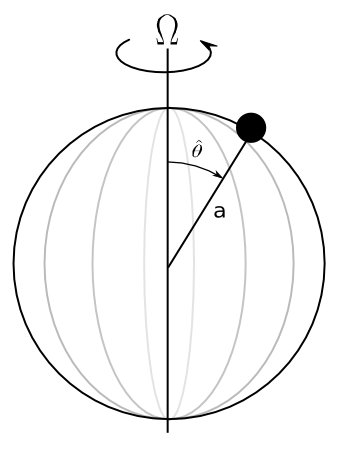
\includegraphics[scale=0.5]{Im.png}
	\end{figure}
	
	A massa é livre para percorrer o aro e este gira com velocidade angular $\Omega$ , $a$ é o raio 
	do aro.
	
	Usando como Coordenada generalizada $\theta$, podemos calcular as Energias:
	
	\[ T = \frac{1}{2} m  (a^2 \dot\theta^2 + a^2 \sin^2(\theta) \Omega^2) \quad \text{,} \quad V = mga\cos{(\theta)}\]
	
	\[\mathcal{L} = T - V \quad \text{então} \quad \mathcal{L} = \frac{1}{2}ma^2 \dot\theta^2 + \Big(\frac{1}{2}ma^2 \sin^2(\theta) \Omega^2 - mga\cos{(\theta)\Big)} \]
	Aqui, Já podemos analisar o potencial efetivo (entre parenteses na Lagrangiana)
	\begin{figure}[h]
		\centering
		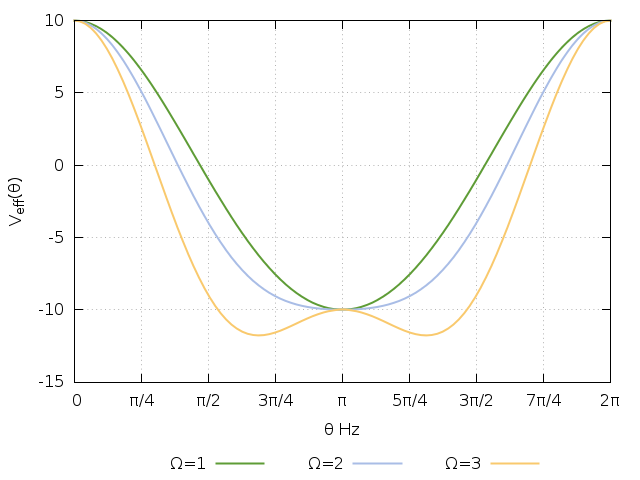
\includegraphics[scale=0.5]{Gr.png}
		\caption{Potencial efetivo }
	\end{figure}
	\\
	Usando a Equação de Euler-Lagrange:
	\[ \frac{d}{dt} \frac{\partial \mathcal{L}}{\partial \dot q_i}  - \frac{\partial \mathcal{L}}{\partial q_i} = 0 \]
	
	Aqui podemos derivar duas equações de movimento uma para $\theta$ e outra para $\Omega$ nesta primeira análise vamos manter $\Omega$ constante
	
	\[ m a^2 \ddot\theta + \frac{1}{2} ma^2\Omega^2 \sin(2\theta) + mga \sin(\theta) = 0\]
	
	\[ \ddot\theta + \frac{1}{2} \Omega^2 \sin(2\theta) + \frac{g}{a} \sin(\theta) = 0\]
	
	e a Equação de movimento para $\theta$ fica:
	\[ \ddot\theta = \sin(\theta)\Big( \frac{g}{a} + \Omega^2 \cos(\theta) \Big) \]
	
	\begin{figure}[h]
		\centering
		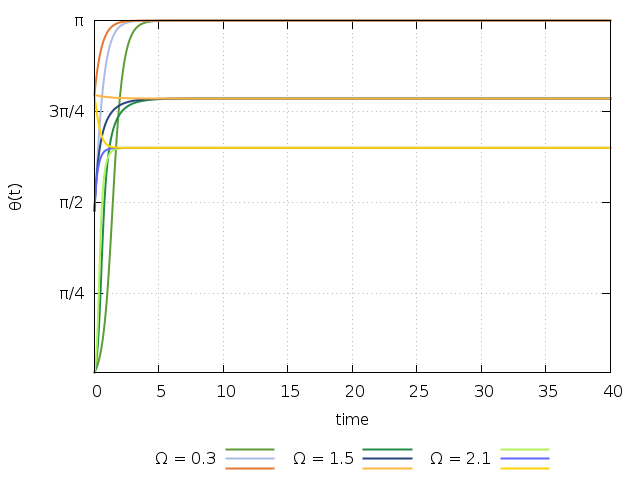
\includegraphics[scale=0.5]{Gr1.png}
		\caption{ $\theta(t)$ Solução Numerica por Runge Kutta, $g=10$, $a=5$}
	\end{figure}
	
	Podemos encontrar a condição para o equilibrio da massa em um angulo qualquer $\theta_0$
	\[ \ddot\theta  = 0 \quad \to \quad \cos(\theta_0) = -\frac{g}{a\Omega^2} \quad \text{ , } \quad \theta_0 = 0 \quad \text{ e } \quad \theta_0 = \pi\]
	\\
	Podemos analisar esses pontos de equilibrio fazendo $\theta(t) = \theta_0 + \delta(t)$ onde $\delta(t)$ é tão pequena quanto quisermos.
	\\
	\begin{itemize}
		
		\item{para $\theta_0$ em torno de $0$.}
		
		\[ \theta(t) = 0 + \delta(t) \quad \to \quad \ddot\theta = \ddot\delta \]
		
		\[ \ddot\delta = sin(\delta)\Big( \frac{g}{a}  +\Omega^2 \cos(\delta) \Big) \]
		
		Expandindo em taylor o seno e o cosseno de $\delta$ 	
		
		\[ \ddot\delta=\Big[\delta-\frac{\delta^3}{3!}+\frac{\delta^5}{5!}-...\Big]\Big[\frac{g}{a}+\Omega^2\big(1-\frac{\delta^2}{2!}+\frac{\delta^4}{4!}-...\big)\Big]\]
		Fazendo $\delta^n \to 0$ para $n>1$ obtemos uma equação muito bem comportada como segue:
		\[ \ddot\delta = \delta \Big( \frac{g}{a}  +\Omega^2 \Big) \quad \text{ ou } \quad \ddot\delta = \alpha^2 \delta\]
		Que tem solução:
		\[ \delta(t) = e^{\alpha t} \quad \text{para} \quad \alpha = \sqrt{\frac{g}{a}  +\Omega^2 }\]
	O equilibrio é instavel neste ponto pois $\alpha^2$ nunca assume valores negativos o que faz o deslocamento não ser restaurador e torna o ponto um equilibrio instável.
		\begin{figure}[h]
			\centering
			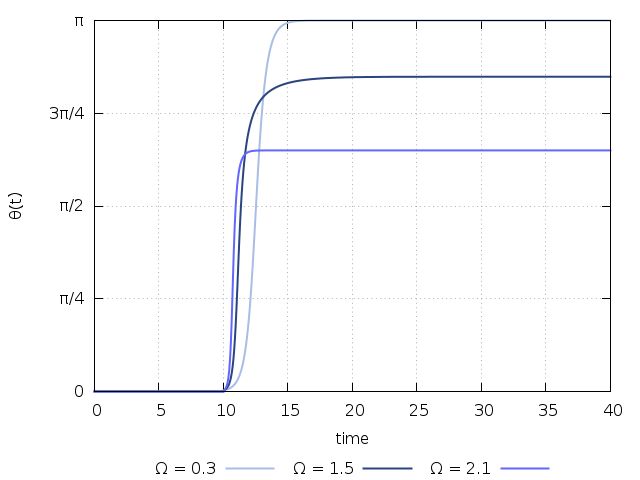
\includegraphics[scale=0.5]{Gr2.png}
			\caption{Teste de Instabilidade, em t=10s a particula sofre um deslocamento de $0.01rad$ na sua posição instantânea}
		\end{figure}
		
		\item{para $\theta_0$ em torno de $\pi$.}
		
		\[ \theta(t) = \pi + \delta(t) \quad \to \quad \ddot\theta = \ddot\delta \]
		Expandindo em taylor o seno e o cosseno de $\pi + \delta$ e fazendo a aproximação
		\[ \ddot\delta = -\delta\Big(\frac{g}{a}-\Omega^2\Big) \quad \text{ ou } \quad \ddot\delta = -\beta^2 \delta\]
		Esta equação pode ser resolvida como:
		\[ \delta(t) = e^{i\beta t} \quad \text{para} \quad \beta = \sqrt{\frac{g}{a}-\Omega^2} \]
		Aqui o equilibrio é estável em $\theta = \pi$, se $\beta^2 > 0$.
		\\
		\pagebreak
		Caso, $ \Omega^2 > g/a $ o equilibrio passa a ser instável nesse ponto também.
		
		\begin{figure}[h]
			\centering
			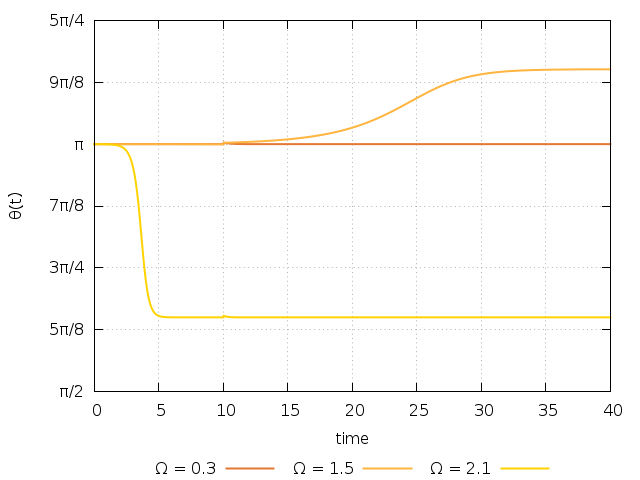
\includegraphics[scale=0.5]{Gr3.png}
			\caption{Teste de Instabilidade, em t=10s a particula sofre um deslocamento de $0.01rad$ na sua posição (Resultado Numérico, para $\Omega$ muito grande não é necesário forçar o deslocamento, o equilibrio é instável com a aproximação de Runge-Kutta consultar código para mais informações)}
		\end{figure}

		\item{ Para $cos(\theta_0) = - \frac{g}{a\Omega^2}$ }

		Voltando a Equação de movimento,  podemos analizar a Força Efetiva ! e poderiamos ter feito isso para os dois casos acima.
		\[ ma^2\ddot\theta = ma^2\sin(\theta)\Big( \frac{g}{a} + \Omega^2 \cos(\theta) \Big) \]
		Onde o termo da direita vamos chamar de Força Efetiva ( $ \tilde F(\theta) $ ) como a Força pode ser escrita como $\tilde F(\theta) = - \frac{\partial \tilde V(\theta)}{\partial \theta}$ e estamos procurando vales de potencial, ao derivarmos a força novamente podemos encontrar a concavidade de cada ponto de equilibrio do sistema e isso nos diz se esse ponto é um ponto de equilibrio estável ou instável dependendo do sinal de derivada de $\tilde F(\theta)$ com relação a $\theta$.
		
	\[ \frac{d \tilde F(\theta)}{d\theta} =\frac{d}{d\theta} \Bigg( ma^2\sin(\theta)\Big( \frac{g}{a} + \Omega^2 \cos(\theta) \Big) \Bigg) \]
	
	\[ \frac{d \tilde F(\theta)}{d\theta} = ma^2\cos(\theta) \Big( \frac{g}{a} + \Omega^2 \cos(\theta) \Big) - ma^2\Omega^2 \sin^2(\theta) \]
	
	\[ \frac{d \tilde F(\theta)}{d\theta} = ma^2\cos(\theta) \Big( \frac{g}{a} + \Omega^2 \cos(\theta) \Big) - ma^2\Omega^2 \Big( 1 - \cos^2(\theta) \Big) \]
	
	\[ \frac{d \tilde F(\theta)}{d\theta} = ma^2\cos(\theta)\frac{g}{a} + ma^2\Omega^2 \cos^2(\theta) - ma^2\Omega^2 + ma^2\Omega^2\cos^2(\theta) \]
	
	\[ \frac{d \tilde F(\theta)}{d\theta} = ma^2\cos(\theta)\frac{g}{a} + 2ma^2\Omega^2 \cos^2(\theta) - ma^2\Omega^2 \]
	
	Substituindo a condição inicial $\cos(\theta_0) = - \frac{g}{a\Omega^2}$ ficamos com:
	
	\[ \frac{d \tilde F(\theta)}{d\theta} \Bigg|_{\theta_{0}} = ma^2 \Big( \frac{g^2}{a^2\Omega^2} - \Omega^2 \Big) \]
	$\theta_0$ é um ponto de equilibrio estável se a equação $\frac{d \tilde F(\theta)}{d\theta} \Bigg|_{\theta_{0}}$ for maior que zero. Caso contrario o equilibrio é instável, portanto.
	
	\[ \quad \frac{g}{a\Omega^2}
	\begin{cases}
	 	 > 1 & \text{Estável} \\ 
	 	 < 1 & \text{Instável} 
	 \end{cases}
	\]
	\begin{figure}[h]
			\centering
			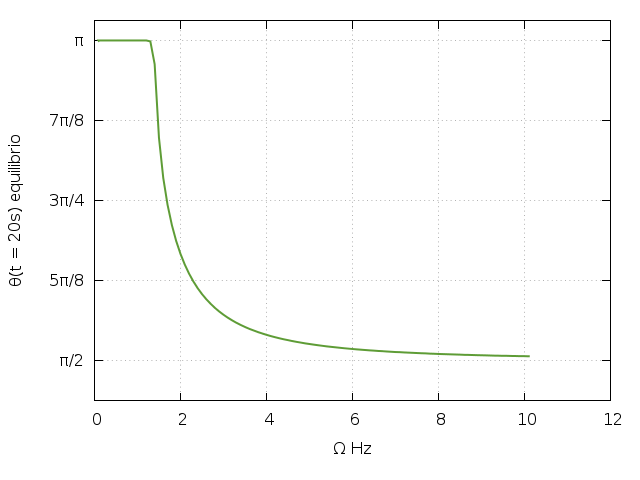
\includegraphics[scale=0.5]{Gr4.png}
			\caption{Posição de Equilibrio em função de $\Omega$}
		\end{figure}
	\end{itemize}
	
	Vamos agora calcular a Hamiltoniana $\mathcal{H}$ para esse sistema, usando$ p(q_i,\dot q_i ,t) = \frac{\partial \mathcal{L}}{\partial \dot q_i}$ e aplicando a transformação de legendre para $\mathcal{L}$.
	\[ \mathcal{H} = \sum_i \dot q_i \frac{\partial \mathcal{L}}{\partial \dot q_i} - \mathcal{L} \quad \text{onde} \quad \frac{\partial \mathcal{L}}{\partial \dot \theta} = ma^2 \dot\theta\]
	
	\[ \mathcal{H} = m a^2 \dot\theta^2  - \mathcal{L} = \frac{1}{2} m(a^2 \dot\theta^2 - a^2 \sin^2(\theta) \Omega^2) - mga\cos{(\theta)} \]
	
	e assim obtemos as equações de Hamilton para o sistema:
	
	\[\dot p_\theta = - \frac{\partial \mathcal{H}}{\partial \theta } = ma^2 \cos(\theta)\sin(\theta)\Omega^2 - mga\sin{(\theta)}\]	
	
	\[\dot \theta = \frac{\partial \mathcal{H}}{\partial \theta } = -ma^2 \cos(\theta)\sin(\theta) \Omega^2 + mga\sin{(\theta)}  \]
	
	Podemos plotar o espaço de fase para a variação de $\Omega$ como segue:
	
	\begin{figure}[h]
			\centering
			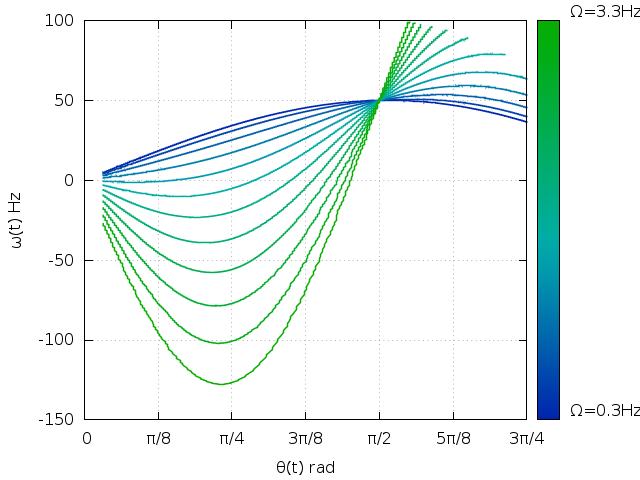
\includegraphics[scale=0.5]{Gr5.png}
			\caption{Espaço de Fase para $\Omega$ variando de $0.3Hz$ a $3.3Hz$ com $\theta_0 = 0.2$ ($\dot\theta$ x $\theta$)}
		\end{figure}
		
	Agora só falta calcularmos a força que atua no aro, e para isso vamos utilizar os multiplicadores de lagrange.\\
	Voltemos na Lagrangeana porém sem introduzir o vínculo:
	
	\[ T = \frac{1}{2} m(r^2 \dot\theta^2 + r^2 \sin^2(\theta) \Omega^2 + \dot r^2) \quad \text{,} \quad V = mgr\cos{(\theta)}\]
	
	\[\mathcal{L} = \frac{1}{2}mr^2 \dot\theta^2 + \frac{1}{2}mr^2 \sin^2(\theta) \Omega^2 + \frac{1}{2} m \dot r^2 - mgr\cos{(\theta)} \]
	Escrevendo explicitamente o vínculo, a massa está restrita a se mover sobre o aro de raio a.
	\[ r = a \quad \to \quad f(r,\theta) = r \quad \text{é a equação do vínculo nesse caso} \]
	E com isso.

	\[ \frac{d \quad \partial \mathcal{L}}{dt\quad \partial \dot q_\sigma} - \frac{\partial \mathcal{L}}{\partial q_\sigma}  - \lambda \frac{\partial f(r,\theta)}{\partial q_\sigma} =0 \]
	desse modo, $\frac{\partial}{\partial r} r = 1 \quad \frac{\partial}{\partial \theta} r = 0$ , com isso podemos escrever, 
	\[\frac{d \quad \partial \mathcal{L}}{dt\quad \partial \dot r} - \frac{\partial \mathcal{L}}{\partial r}  - \lambda_r = 0  \]
	
	\[\frac{d \quad \partial \mathcal{L}}{dt\quad \partial \dot \theta} - \frac{\partial \mathcal{L}}{\partial \theta} = 0  \]
	
	\[ m \ddot r  - mr\dot \theta -mr\sin^2(\theta) \Omega^2 + mg\cos(\theta) = \lambda_r \equiv Q_r\]
	\[ 2m r \dot r \ddot \theta  - mr^2\sin(2 \theta) -mgr\sin(\theta) = 0\]
	Podemos interpretar as equações e analisar os gráficos para a força e compara-los com o potencial efetivo
	\[ Q_r = m( \ddot r  - r\dot \theta - r\sin^2(\theta) \Omega^2 + g\cos(\theta) ) \]
	\[ \ddot \theta = \frac{\sin(\theta)}{2 \dot r} (r \cos(\theta) + g)\]
	Introduzindo o vínculo novamente reduzimos a equação de $Q_r$ para
	\[ Q_r = -ma \dot \theta -ma\sin^2(\theta)\Omega^2 + g \cos(\theta) \]
	Usando Runge-Kutta podemos plotar $Q_r$ em função de $\theta$. pois o termo que vai com $\dot \theta$ é simplesmente a primeira parte da recurssão em Runge-Kutta
	
	\begin{figure}[h]
			\centering
			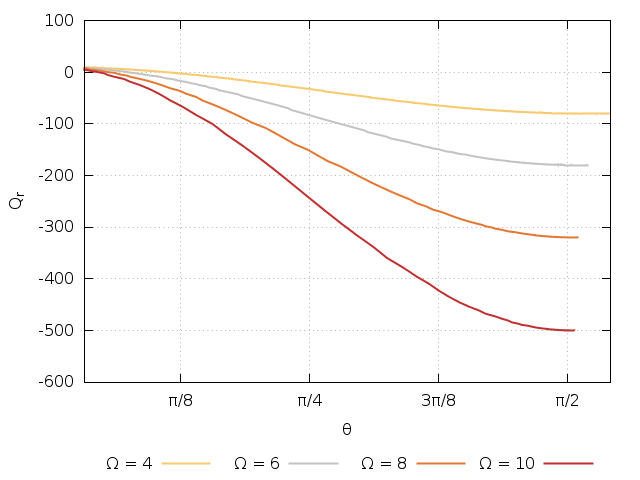
\includegraphics[scale=0.35]{Gr6.png}
			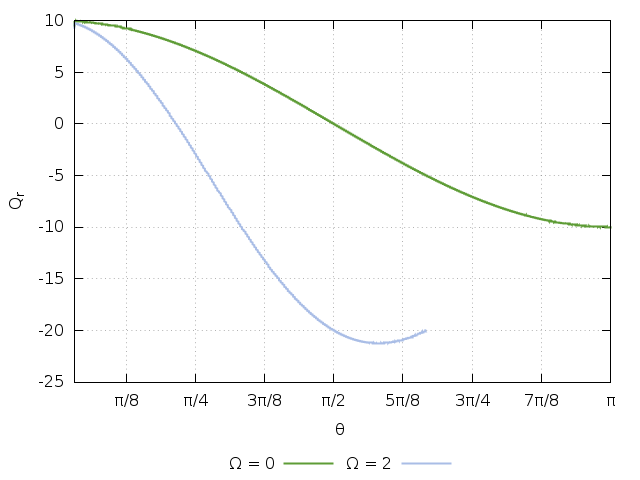
\includegraphics[scale=0.35]{Gr7.png}
			\caption{Forças Generalizadas $Q_r$ para diferentes $\Omega s$}
	\end{figure}
	
	\pagebreak
	
	\begin{lstlisting}	
	
	## Runge-Kutta de quarta ordem , essa funcao sera usada em todos os coidigos
	
def RK4(f):
    return lambda t, y, dt: (
            lambda dy1: (
            lambda dy2: (
            lambda dy3: (
            lambda dy4: (dy1 + 2*dy2 + 2*dy3 + dy4)/6
            )( dt * f( t + dt  , y + dy3   ) )
	    )( dt * f( t + dt/2, y + dy2/2 ) )
	    )( dt * f( t + dt/2, y + dy1/2 ) )
	    )( dt * f( t       , y         ) )
	    
	\end{lstlisting}
	Para o Calculo de $\theta$ (Figure 2)
	\begin{lstlisting}	
from math import sin, cos
import sys

## (y deve ser interpretado como theta aqui dentro!)
## argumantos passados na chamada do programa , y0 = theta inicial
## O2 = Omega (velocidade angular do aro)

if len(sys.argv) > 2:
	y0 = float(sys.argv[1])
	O2 = float(sys.argv[2])
else:
	y0 , O2, = 0.001 , 2
	
## g = 10
## a = 5
g,a = 10, 5

## Chamada da RK4 com a equacao diferencial inicial.
dy = RK4(lambda t, y: sin(y)*((g/a) + pow(O2,2)*cos(y)))

## Condicoes iniciais para tempo theta (y0) e dt
t, y, dt = 0., y0, .01

## Condicao de parada
TMAX = 40

########## Variacoes de codigo ocorrem apenas daqui para baixo ##########
#*
while t <= TMAX:
	print("%2.2f \t %4.6f " % (t, y))
	## Passagem Recursiva dos parametros da funcao "dy" 
	## para atingir a segunda ordem em y
	t, y = t + dt, y + dy( t, y + dy( t, y, dt ), dt )
	\end{lstlisting}
Para o Grafico de $\theta_0$ equilibrio em função de $\Omega$ (Figure 5)
	\begin{lstlisting}	
from math import sin, cos
import sys

if len(sys.argv) > 2:
	y0 = float(sys.argv[1])
	O2 = float(sys.argv[2])
else:
	y0 , O2, = 0.001 , 0
	
g,a = 10, 5

TMAX = 20

while O2 <= 10:
	dy = RK4(lambda t, y: sin(y)*((g/a) + pow(O2,2)*cos(y)))
	t, y, dt= 0., y0, .01
	O2 = O2 + 0.1
	## Calcula ate o ultimo valor de theta e so depois da o print do valor de omega com o theta final
	while t <= TMAX:
		t, y = t + dt, y + dy( t, y + dy( t, y, dt ), dt )
	print("%2.2f \t %4.6f " % (O2, y))	
	\end{lstlisting}
	Para os testes de instabilidade uma pequena variação no primeiro código (Figure 3 e Figure 4)
	\begin{lstlisting}
from math import sin, cos
import sys

if len(sys.argv) > 2:
	y0 = float(sys.argv[1])
	O2 = float(sys.argv[2])
else:
	y0 , O2, = 0.001 , 2
	
g,a = 10, 5


dy = RK4(lambda t, y: sin(y)*((g/a) + pow(O2,2)*cos(y)))

t, y, dt = 0., y0, .01
TMAX = 40

while t <= TMAX:
	## Variacao em theta quando o tempo esta em 10s
	if (t > 10 and t < 10 + dt): #Condicao para um pequeno deslocamento em t = 10s
		y=y+0.01
		t = t+dt
	else:
		print("%2.2f \t %4.6f " % (t, y))
		t, y = t + dt, y + dy( t, y + dy( t, y, dt ), dt )
	\end{lstlisting}
	
Para o Espaço de Fase (Figure 6)
	
	\begin{lstlisting}
from math import sin, cos
import sys

if len(sys.argv) > 2:
	y0 = float(sys.argv[1])
	O2 = float(sys.argv[2])
else:
	y0 , O2, = 0.001 , 4
	
g,a = 10, 5
m=1

dy = RK4(lambda t, y: sin(y)*((g/a) + pow(O2,2)*cos(y)))

t, y, dt = 0., y0, .001

while t <= 10:
	p = -m*pow(a,2)*cos(y)*sin(y)*pow(O2,2) + m*g*a*sin(y)
	#if abs(round(t) - t) < 1e-5:
	print("%2.2f \t %4.6f " % (y,p))
	t, y = t + dt, y + dy( t, y + dy( t, y, dt ), dt )
	\end{lstlisting}
		
Para as Forças generalizadas $Q_r$ (Figure 7)
	
	\begin{lstlisting}
from math import sin, cos
import sys

if len(sys.argv) > 2:
	y0 = float(sys.argv[1])
	O2 = float(sys.argv[2])
else:
	y0 , O2, = 0.001 , 2
	
g,a = 10, 5
m=1

dy = RK4(lambda t, y: sin(y)*((g/a) + pow(O2,2)*cos(y)))

t, y, dt = 0., y0, .001
## dy/dt e a velocidade angular com que a conta oscila no aro calculado na primeira ordem 
dydt = 0
Qr = g*cos(y) - m*a*y - m*a*pow(sin(y),2)*pow(O2,2)
while t <= 10 :

	print("%2.2f \t %4.6f " % (y , Qr))
	t, y = t + dt, y + dy( t, y + dy( t, y, dt ), dt )
	
	t, dydt = t + dt, dydt + dy( t, dydt, dt )
	Qr = g*cos(y) - m*a*dydt - m*a*pow(sin(y),2)*pow(O2,2)
	
	\end{lstlisting}
\end{document}
